% Theorie: Physikalische Grundlagen von Versuch/Messverfahren, Gleichungen ohne Herleitung knapp erklären
\section{Theorie}
\label{sec:theorie}

Im Folgenden werden elementare Begriffe der Strahlen- und der Wellenoptik eingeführt und erläutert.

Licht ist eine Form der elektromagnetischen Strahlung. Das optische Spektrum erstreckt sich von ultraviolettem Licht, welches 
in einem Wellenlängenbereich von $\SI{100}{\nano\meter}$ bis $\SI{380}{\nano\meter}$ vorkommt und reicht bis in das Infrarotspektrum, welches 
den Wellenlänenbereich von $\SI{780}{\nano\meter}$ bis $\SI{1}{\milli\meter}$ hat. Das für den Menschen sichtbare Licht ist dabei in dem 
Wellenlängenbereich von $\SI{380}{\nano\meter}$ bis $\SI{780}{\nano\meter}$.

\subsection{Strahlenoptik}
\label{sec:Strahlenoptik}
 
Für die Beschreibung von Refelxion und Brechnung an Grenzflächen können die Regeln der Strahlenotik angewandt werden.
Dabei wird die Wellenausbreitung über die Normalen der Wellenflächen beschrieben. Diese wird als Lichtstrahl bezeichnet.
Lichtstrahlen breiten sich in einem homogenen Medium gradlinig aus. Wenn sich zwei oder mehr Lichtstrahlen kreuzen haben diese
keine Einflüsse aufeinander.
Für unterschiedliche Materialien ist auch die Ausbreitungsgeschwindigkeit der Welle anders. Daher wird beim Übergang von einem
Medium in ein anderes die Welle gebrochen. Für die Aubreitungsgeschwindigkeiten $v_1$ und $v_2$ ergibt sich die Beziehung
\begin{equation}
    \frac{\sin \alpha}{\sin \beta} =\frac{v_1}{v_2} = \frac{n_1}{n_2}.
    \label{eqn:bez}
\end{equation}
Dabei beschreibt der Winkel $\alpha$ den Einfallswinkel und $\beta$ den Ausfallswinkel, beide Winkel werden  zur Normalen der Grenzfläche gemessen. 
$n$ ist der Brechungsindex, welcher eine optische Materialeigenschaft ist.
Wenn die Ausbreitungsgeschwindigkeit in Medium 1 größer ist als die in Mediu  2, wird das Medium 1 als optisch dünner 
bezeichnet. Andersherum ist das Medium 1 optisch dicker.

\subsubsection{Reflexion}
\label{sec:Reflexion}
Für einen reflektierten Lichtstrahl, welche in \autoref{fig:bild1} zu sehen ist, gilt
\begin{equation}
    \alpha_1 = \alpha_2
    \label{eqn:relex}
\end{equation}

    \begin{figure}[H]
    \centering
	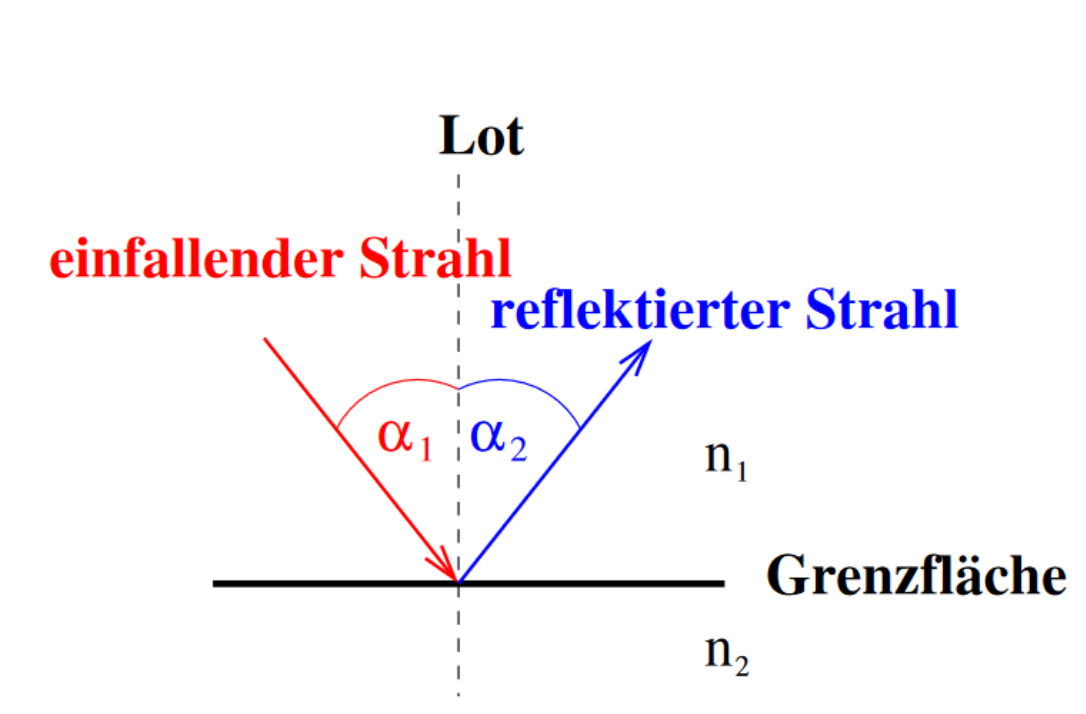
\includegraphics[width=0.6\linewidth]{content/grafik/reflexion.png}
	\caption{Refelxion an einer Grenzfläche. \cite{reflex}}
	\label{fig:bild1}
\end{figure}

\subsubsection{Brechung}
\label{sec:Brechung}
Wenn ein Lichtstrahl auf ein anderes Medium mit dem Brechungsindex $n$ trifft, ändert sich die Ausbreitungsgeschwindigkeit
des Lichtstrahls in diesem. Der Lichtstrahl erfährt einen Richtungswechsel, sobald diese an der Grenzfläche auftrifft.
Diese Richtungsänderung wird als Brechung bezeichnet, dies ist in \autoref{fig:bild2} dargestellt. Es gilt das Gesetz nach Snellius
\begin{equation}
  n_1  \cdot \sin \alpha_1 = n_2 \cdot \sin \alpha_2.
\end{equation}

\begin{figure}[H]
    \centering
	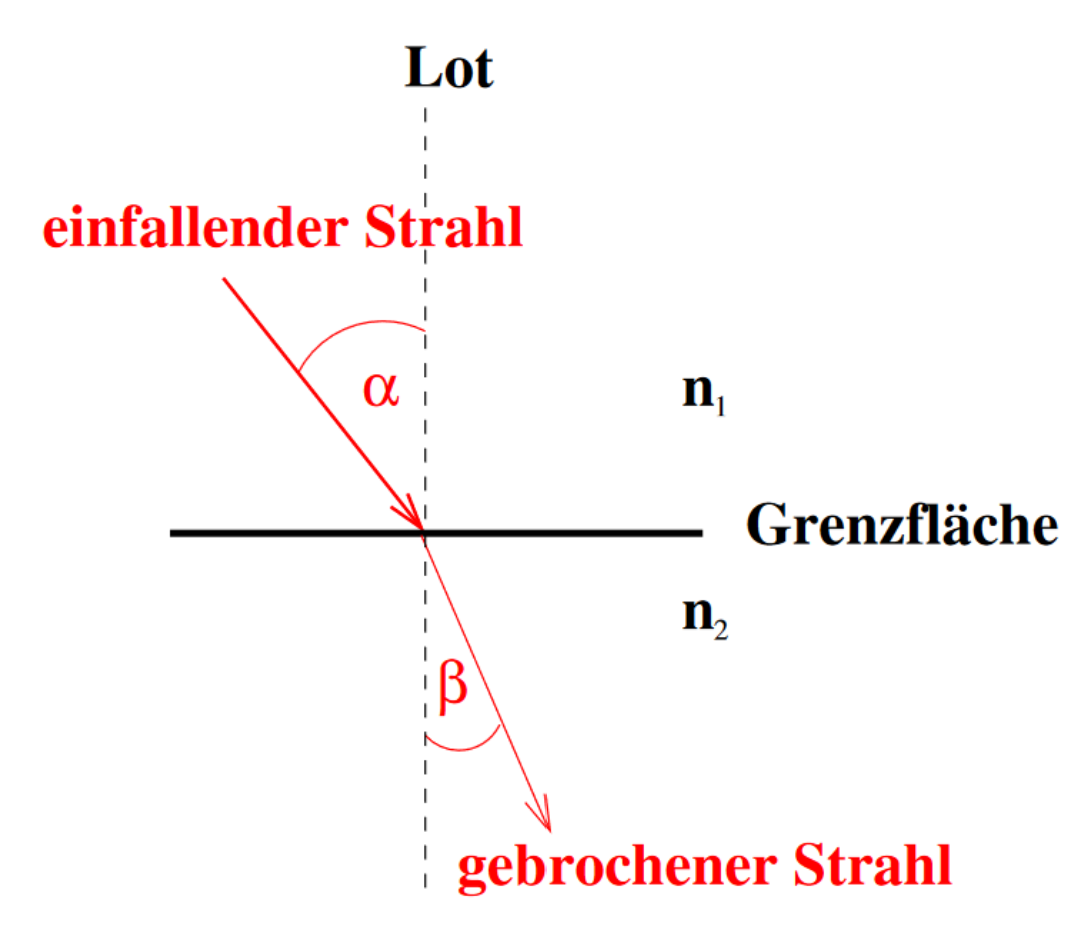
\includegraphics[width=0.6\linewidth]{content/grafik/brechung.png}
	\caption{Brechnung an einer Grenzfläche. \cite{reflex}}
	\label{fig:bild2}
\end{figure}

\subsubsection{Reflexion und Transmission}
\label{sec:Reflexion und Transmission}
Normalerweise wird ein Lichtstrahl an einer Grenzfläche nicht ausschließlich relektiert beziehungsweise gebrochen.
Daher wird ein Teil der Intensität $R$ relektiert und der andere Teil $T$ wird gebrochen und transmittiert. Siehe \autoref{fig:bild3} 
Es gilt immer $R + T = 1$.

\begin{figure}[H]
    \centering
	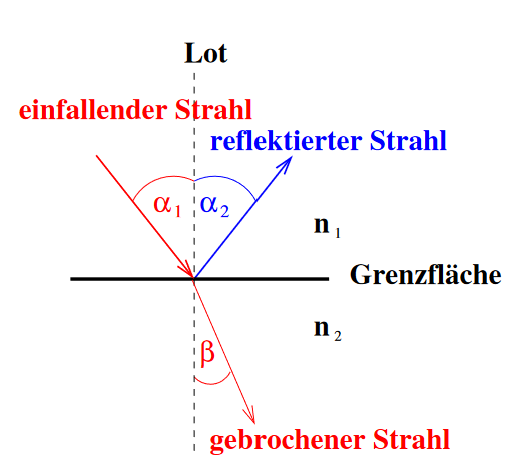
\includegraphics[width=0.6\linewidth]{content/grafik/trans.png}
	\caption{Refelxion und Transmission an einer Grenzfläche. \cite{reflex}}
	\label{fig:bild3}
\end{figure}

\subsection{Wellenoptik}
\label{sec:Wellenoptik}
Es kann beobachtet werden, dass Licht sich im Schattenraum ausbreitet, wenn dieses auf ein Hindernis trifft.
Dieses Phänomen wird als Beugung bezeichent und kann nicht mit der Strahlenoptik erklärt werden.  Daher wird 
für die Erklärung die Wellenoptik herangezogen. Charakteristisch für eine elektromagnetische Welle ist die Frequenz $\nu$
und die Wellenlänge $\lambda $ und die Ausbreitungsgeschwindigkeit $v$ der Welle. Bei der Überlagerung von zwei oder mehreren Wellen, 
kommt es zur Superposition derer Amplituden. Licht besteht aus vielen Wellenzügen, wen diese Wellenzüge dieselbe Frequenz und eine
feste Phasenbeziehung haben, kommt es zu einem Interferenzbild. Je nach Phasenbeziehung kommt es zu einer Verstärkung, also 
einer konstruktiven Interferenz oder zu eine Abschwächung, einer destruktiven Interferenz. Zwei Wellen löschen sich vollkommen aus,
wenn der Gangunterschied $\lambda/2$ ist und die Intensitäten gleich sind. Die Ausbreitung einer Welle wird über das Huygensche
Prinzip konstruiert. Dieses besagt, dass jeder Punkt einer Welle  der Ausgangspunkt einer Elementarwelle gleicher Frequenz ist.
Außerdem ist die Einhüllende aller Sekundarwellen zu einem späteren Zeitpunkt die neue Position der Wellenfront.

\subsubsection{ Beugung am Einzelspalt}
\label{sec:Beugung am Einzelspalt}

Trifft eine Wellenfront auf einen Spalt mit der Spaltbreite $a$ , so werde  alle Punkte dieser an der Spaltöffnung gebeugt.
Für die gebeugten Wellen gilt die gleiche Frequenz und die gleiche Phasenbeziehung. In einem Abstand $L$ wird ein 
Schrim plaziert. Auf diesem können dunkle und helle Interfrenzstreifen beobachtet werden. Für die hellen Maxima kann gesagt 
werden, dass diese an Stellen auftreten , für die gilt
\begin{equation}
    \alpha \sin \alpha = k \lambda.
\end{equation}

\subsubsection{ Beugung am Gitter}
\label{sec:Beugung am Gitter}

Ein Mehrfachspalt oder auch Gitter genannt, besteht aus N-Einfachspalten gleicher Breite. Fällt eine Wellenfront
senkrecht auf ein Strichgitter mit der Gitterkontsante $d$ , können Bedingungen für Intensitätsminima und Intensitätsmaxima
aufgestellt werden.
Für die Intensitätsmaxima $k$-ter Ordnung gilt
\begin{equation}
    d \sin \alpha = k \lambda.
\end{equation}